\section{Processi organizzativi}
\subsection{Processo di coordinamento}
\subsubsection{Comunicazioni}
Le comunicazioni possono essere interne o esterne al \termine{team}.

\paragraph{Comunicazioni interne}
Dipendentemente dal carattere della comunicazione, si deve decidere se effettuarle in modo formale o informale.
In funzione di questi due criteri, le forme di comunicazione che vengono adottate sono:
\begin{itemize}
	\item \textbf{Comunicazione formale scritta}: le informazioni comunicate in questa forma hanno carattere ufficiale, e avranno quindi una grande importanza per il \termine{team}.
	\item \textbf{Comunicazione verbale formale}: comunicazioni divulgative o di presentazione.
	\item \textbf{Comunicazione informale scritta}: discussioni tra membri del \termine{team} non ufficiali, al fine di chiarire dubbi o fare proposte senza ufficialità.
	\item \textbf{Comunicazione informale orale}: informazioni non ufficiali scambiate tra i membri del \termine{team} riguardanti il progetto.
\end{itemize}

Per ogni tipologia di comunicazione si è deciso di utilizzare i seguenti strumenti:
\begin{itemize}
	\item \textit{\PdP}, convocazioni di riunione e verbali di riunione per le comunicazioni formali scritte.
	\item Presentazioni e discorsi per le comunicazioni verbali formali.
	\item Piattaforme di \termine{instant messaging} per le comunicazioni informali scritte.
	\item Conversazioni per le comunicazioni informali orali.
\end{itemize}

La comunicazione interna viene usata dal \termine{team} per:
\begin{itemize}
\item
Trasmettere informazioni su scadenze e obiettivi tecnici.
\item
Informare i membri del \termine{team} sull'organizzazione.
\item
Motivare i membri del \termine{team}.
\end{itemize}

\paragraph{Comunicazioni esterne}
Per le comunicazioni esterne è stata creata la seguente casella di posta elettronica:

\begin{center} \email \end{center}

Il \Pm gestisce le comunicazioni con i proponenti e i committenti, avvertendo i membri del \termine{team} nel caso vengano rese disponibili nuove informazioni utili.


\subsection{Processo di pianificazione}
\subsubsection{Descrizione}
Nell'arco dello sviluppo del progetto ogni membro del gruppo dovrà assumere almeno una volta tutti i ruoli progettuali.
Un membro del \termine{team} può assumere più ruoli contemporaneamente, ma non può mai essere redattore e verificatore dello stesso documento, al fine di evitare conflitti di interesse che potrebbero vanificare il processo di verifica del materiale prodotto.

\paragraph{\Pm}
Il \Pm\ rappresenta l'intero \termine{team} in situazioni formali come la comunicazione con i committenti e i proponenti. È anche il responsabile ultimo del lavoro del gruppo. Inoltre redige l'\termine{organigramma}, assegnando task e scadenze ai membri del \termine{team}, assicurandosi che queste vengano soddisfatte. 
Il \Pm\ approverà definitivamente i documenti, oltre che a collaborare alla stesura del \PdP\  e del \PdQ.
Infine elabora ed emette piani per il \termine{team}.

\paragraph{\Am}
L'\Am\ si occupa dell'ambiente di sviluppo del \termine{team}. Più in dettaglio, egli si occupa di:
\begin{itemize}
  \item Controllo dell'ambiente di lavoro.
  \item Gestione del versionamento della documentazione.
  \item Controllo delle versioni e delle configurazioni del prodotto.
\end{itemize}
L'\Am\ redige le \NdP\ e collabora alla stesura del
\PdP.

\paragraph{\Prog} 
Il \Prog\ è il responsabile di tutto ciò che riguarda la progettazione.
Più in dettaglio, egli si occupa di:
\begin{itemize}
  \item Produrre una soluzione attuabile, robusta e semplice entro i limiti di
  tempo stabiliti.
  \item Garantire la manutenibilità e la modularità del prodotto software.
\end{itemize}
Il \Prog\ redige la \ST, la \DDP\ e la parte
programmatica del \PdQ.

\paragraph{\An}
L'\An ha il dovere di scomporre il problema in parti sempre più elementari che lo portino ad una comprensione completa del problema iniziale.
Il frutto del suo lavoro serve al progettista per costruire una soluzione che davvero risponda alle aspettative dei committenti.
In dettaglio l' \An\ deve produrre una specifica di progetto comprensibile per il \termine{proponente}, per il \termine{committente} e per il \Prog. \\
L'\An\ redige lo \SdF, l'\AdR\ e parte del \PdQ.

\paragraph{\Ver}
Il \Ver\ è responsabile della qualità del lavoro del \termine{team}.
Egli effettua la verifica dei documenti e del software utilizzando gli strumenti e i metodi proposti nel
\PdQ\ e seguendo rigorosamente quanto descritto nelle \NdP.
Egli ha il compito di garantire la conformità rispetto le \NdP\ dei documenti e del software da lui verificati.

\paragraph{\Progr}
Il \Progr\ ha la responsabilità di implementare le soluzioni del \Prog, e quindi è
responsabile dell'attività di codifica. In dettaglio, i suoi compiti sono:
\begin{itemize}
  \item Implementare le soluzioni descritte dal \Prog\ in maniera rigorosa.
  \item Scrivere il codice rispettando le convenzioni prese nelle \NdP.
  \item Implementare i test per il codice scritto da utilizzare per l'attività di verifica.
\end{itemize}
Il \Progr\ redige il \MU e produce la documentazione del codice.

\subsection{Strumenti}
\subsubsection{GitHub}
Gli strumenti per il versionamento rendono possibile lo sviluppo del software in maniera controllata e quantificabile. È stato quindi deciso di creare una \termine{repository} che ospiterà documenti digitali e manuali, oltre che al codice sorgente del software, rendendo possibile il tracciamento della loro evoluzione. \\
Il software di versionamento scelto è \termine{Git} perché presenta molti più aspetti positivi rispetto ad altri sistemi di versionamento centralizzati. \termine{Git} permette ai membri del \termine{team} di copiare la \termine{repository} in locale, lavorandoci anche in assenza di connessione, per poi successivamente caricare nuovamente su di essa i file modificati. \\
Il servizio scelto per l'\termine{hosting} delle \termine{repository} contenenti rispettivamente i documenti, il codice sorgente dell'\termine{SDK} e il codice sorgente della applicazione \termine{demo} è \termine{GitHub} e la loro struttura base è la seguente:
\begin{itemize}
  \item \termine{Repository} dei documenti
  	\begin{itemize}
  		\item RR
			\begin{itemize}
				\item Interni
				\item Esterni
			\end{itemize}
  		\item RQ
  			\begin{itemize}
				\item Interni
				\item Esterni
			\end{itemize}
  		\item RP
  			\begin{itemize}
				\item Interni
				\item Esterni
			\end{itemize}
  		\item RA
  			\begin{itemize}
				\item Interni
				\item Esterni
			\end{itemize}
  		\item Template
  			\begin{itemize}
  				\item Firme
  			\end{itemize}
  	\end{itemize}
  	\item \termine{Repository} del codice sorgente dell'\termine{SDK}
  		\begin{itemize}
  			\item Codice sorgente dell'\termine{SDK}
  		\end{itemize}
  	\item \termine{Repository} del codice sorgente dell'applicazione \termine{demo}
  		\begin{itemize}
  			\item Codice sorgente dell'applicazione \termine{demo}
  		\end{itemize}
  	
\end{itemize}

\paragraph{Regole per il push}
Il team ha standardizzato i \termine{push} da effettuare nella \termine{Repository} contenente i documenti. Dovrà essere specificato il documento (documenti se più di uno) modificati/creati in quel particolare commit. Non è ancora stato definito un metodo unico per i \termine{push} effettuati nella codifica del codice. Esso verrà definito prima dell'inizio dell'attività di codifica.

\subsubsection{Wrike}
\termine{Wrike} è uno strumento online per la collaborazione ed il project management. Permette ai suoi utenti di modificare progetti, classificare le attività per importanza e collaborare con altri utenti dello stesso gruppo. 

\subsubsection{Gestione delle attività del progetto}
Si è scelto di utilizzare il sistema di pianificazione delle attività \termine{Wrike}, grazie al quale vengono tenute sotto controllo le milestones, i task personali e di gruppo. Il programma \termine{Wrike} è disponibile anche come applicazione su sistemi operativi mobile, garantendo più velocità nella comunicazione di eventuali novità nelle attività del gruppo.

\subsubsection{Task management}
I \termine{task} vengono creati dal \Pm\ e possono essere assegnati ad uno o più membri del gruppo. Nel caso in cui il compito sia di particolare importanza, il \Pm\ suddividerà il \termine{task} principale in sotto-task, e li assegnerà ai membri del \termine{team}. Egli, inoltre, dovrà segnare come \textbf{New} tale \termine{task}, e dovrà indicare nella sezione commenti eventuali consigli o informazioni utili al destinatario del task. \\
Successivamente il \Pm\ creerà i sotto-task di verifica assegnandoli ad un verificatore che avrà il compito di appurare la bontà del lavoro compiuto nel \termine{task} superiore, quando questo sarà segnato come pronto per la verifica. \\
Il primo componente che inizierà a lavorare su quel \termine{task} dovrà segnarlo come \textbf{In corso}. \\
Se durante l'elaborazione del \termine{task} arriverà un compito con priorità maggiore al membro che stava lavorando in quel suddetto \termine{task}, l'utente dovrà metterlo in stato \textbf{In sospeso} e completarlo una volta finiti i \termine{task} di maggior priorità
Una volta che il proprietario riterrà il suo sotto-task completato dovrà segnalarlo come \textbf{In sospeso}, in modo tale che il verificatore assegnato possa controllarlo e segnarlo come completato nel caso in cui risultasse idoneo. \\
Se il \termine{task} riguarda la stesura di un documento, una volta completata la verifica, il verificatore dovrà segnarlo come \textbf{In sospeso}, lasciando al \Pm\ la responsabilità dell'ultima verifica e dell'approvazione del documento. A seguito di tale verifica ed approvazione, il \Pm\ segnerà successivamente il task come \textbf{Completato}.
Il ciclo di vita di un task è descritto nel figura 2.0
\label{figura 2.0}
\begin{figure}[ht]
	\centering
	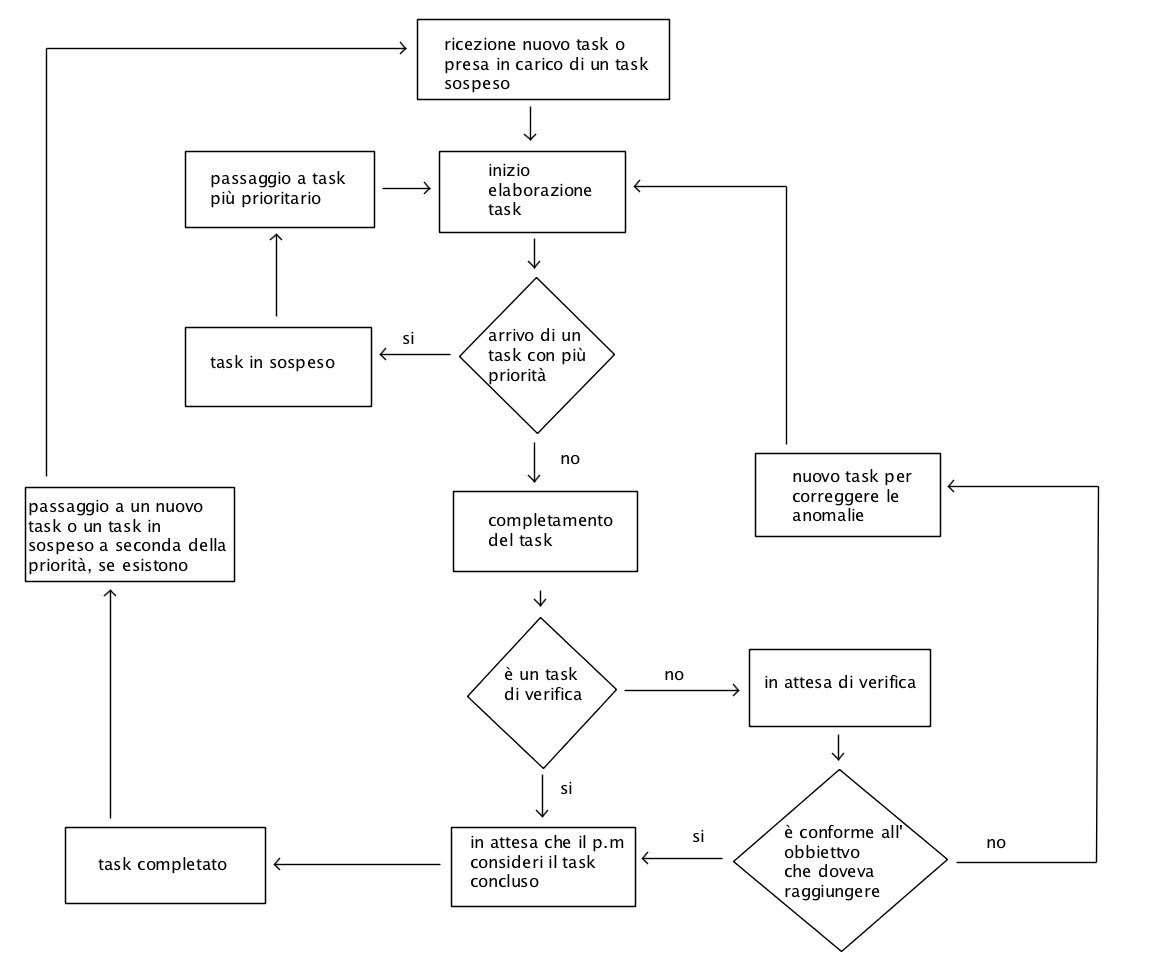
\includegraphics[scale=0.8]{lavorazione_task.jpg}
	\caption{Ciclo di vita di un task}
\end{figure}



\paragraph{Creazione di un task}
Per la creazione di un nuovo singolo \termine{task} bisogna seguire le seguenti
istruzioni:
\begin{enumerate}
  \item Dalla pagina principale di \termine{Wrike} selezionare il progetto interessato (\progetto).
  \item Selezionare la voce \textbf{Nuova attività} e compilare il \termine{task} nel seguente modo:
    \begin{itemize}
      \item \textbf{Nome task:} assegnare un nome identificativo al \termine{task} seguito dalla \termine{milestone} corrispondente (se necessaria).
      \item \textbf{Aggiungi descrizione:} inserire una descrizione breve ma
      concisa del \termine{task}.
      \item \textbf{Allega file:} allegare, eventualmente, file utili alla realizzazione del task.
      \item \textbf{Priorità:} inserire, opzionalmente, una priorità al \termine{task}.
    \end{itemize}
\end{enumerate}


\paragraph{Modifica di un task}
Per modificare un \termine{task} seguire le seguenti istruzioni:
\begin{itemize}
  \item Selezionare il \termine{task} da modificare.
  \item Dalla pagina proposta selezionare il campo che si vuole modificare.
  \item Completata la modifica premere il pulsante \textbf{Invio}.
\end{itemize}

\paragraph{Completamento di un task}
Dopo che il verificatore avrà appurato che il \termine{task} soddisfa i requisiti richiesti, e quindi è stato completato secondo le \NdP, potrà procedere con il suo completamento ottenibile tramite le seguenti operazioni:
\begin{itemize}
  \item Selezionare il \termine{task} da segnare come completato.
  \item Cliccare nella checkbox apposita segnando il termine come \textbf{"Completato"}.
\end{itemize}
Il lavoro viene quindi considerato concluso da questo momento, ma potrebbe essere riportato nello stato \textbf{"In corso"} nel caso in cui:
\begin{itemize}
  \item Il \Pm\ non approvi il documento.
  \item Il \Ver\, dopo un secondo controllo sui \termine{task} a lui assegnati, si accorga di errori e/o incompletezze. 
\end{itemize}

\subsection{Processo di Formazione}
\subsubsection{Descrizione}
Il processo di formazione consiste nel fornire e mantenere tutti i membri del gruppo preparati e in grado di lavorare efficacemente ed efficientemente nella produzione e nella gestione del software.

\subsubsection{Implementazione}
Il \termine{team} ha deciso che la formazione dei membri del gruppo non sarà di pertinenza del gruppo stesso, bensì un dovere del singolo che dovrà intraprendere azioni di autoapprendimento nel caso le sue conoscenze fossero insufficienti al completamento del suo lavoro.

\subsubsection{Materiale di Formazione}
Essendo il processo di formazione riguardante il singolo, ogni membro del \termine{team} che raccolga materiale interessante lo distribuirà all'interno del gruppo. In questo modo il ripresentarsi di problemi di natura similare avrà già parte della soluzione trovata. Eventualmente un membro del \termine{team} può anche chiedere delucidazioni alla persone che in precedenza aveva già trovato una soluzione al medesimo problema.


%
% la parte riguardante la lista di controllo è stata eliminata in quanto
% il prof. stesso ha detto che l improvement dei processi è un processo lungo
% che non riguarda un progetto della durata simile alla nostro
%
%
%\subsection{Lista di controllo}
%Durante l'applicazione della tecnica del \textit{Walkthrough\ped{G}} ai documenti sono stati riportati
%più frequentemente i seguenti errori:
%\begin{itemize}
 % \item\textbf{Norme stilistiche}:
  %\begin{itemize}
   % \item La prima parola di una voce dell'elenco puntato non inizia con una lettera maiuscola.
%    \item La voce dell'elenco puntato termina con un punto anziché con un punto e virgola o viceversa.
 %   \item I due punti in grassetto.
  %  \item Errori di battitura.
    
  %\end{itemize}

  %\item\textbf{Italiano}:
  %\begin{itemize}
   % \item Maiuscole usate impropriamente.
    
  %\end{itemize}

  %\item\textbf{\LaTeX}:
  %\begin{itemize}
  %\item Mancato utilizzo dei comandi \LaTeX{} personalizzati.

  %\end{itemize}
  
  %\item\textbf{Casi d'Uso}:
  %\begin{itemize}
%\item Mancato rispetto del template stabilito per i punti trattati nei casi d'uso.
 % \end{itemize}

	%\item\textbf{Glossario}:
	%\begin{itemize}
	%	\item Sono stati evidenziati dei termini che non andavano nel \textit{\glossario{}}.
	%	\item Non sono stati evidenziati dei termini che sono presenti nel \textit{\glossario{}}.
	%\end{itemize}

%\end{itemize}
